\chapter{Security Policy Models}
\graphicspath{{Chapter3/figures/}}
\label{SecurityPolicyModels}
A security policy is
\begin{quote}
  a set of rules~(or principles) that direct how a system~(or an
  organisation) provides security services to protect sensitive and
  critical system resources~\cite{RS07}.
\end{quote}
A security policy must therefore specify \emph{all} necessary control
measures for ensuring system security, including how authentication
should be done and what responses should be made to a security
violation, etc.

Access control specification is typically a major component of a
security policy. Access control protects the resources of a
system~(objects) against unauthorised access by restricting the use of
system resources only to the authorised users~(subjects) according to
the security policy of the system~\cite{RS07}. Access can be in many
modes; the common ones include read, write, append and execute. The
access mode that a subject has on the objects in the system is known
as the~``privilege'' the subject has. The set of high-level rules that
specifies which accesses are to be authorised and which are not is
known as the access control policy~\cite{PS01}. The study of access
control policies has resulted in various useful models. Most of these
models are formal, i.e., formal analysis can be carried out to prove
the models are secure with respect to the security objectives
concerned. There are also some models consisting of informal
high-level principles such as the Clark-Wilson model~\cite{DDC87}.

This chapter first reviews the traditionally influential security
policies and models in the literature. It then presents some recently
proposed risk-budget based models that aim to provide more
flexibility. Next, it introduces the top-down policy hierarchical
model that enables policy composition and refinement, with an emphasis
on the problems encountered in the refinement and conflict analysis
processes. Lastly, it summarises the current state of the art in
security policy development and reiterates the research objectives of
the thesis.

\subsection{Economics based models}
\label{JASONEconomicsBasedModel}
The idea of managing risk in access control using economic concepts is
proposed in~\cite{JPO04}. Each user in an organisation is allocated a
number of risk tokens, which can be spent for operational needs. The
number of risk tokens a user will get in the future depends on the
return of investment of the user. Essentially, risk is viewed as a
type of limited resource in an organisation and the access control
problem is transformed into a resource allocation problem. Two
economics based models are introduced: one based on the command
economic system and the other based on the market economic system.

% The proposal is done in three incremental phases. The first phase is
% the preparatory phase, where the necessary components in making the
% system work are discussed. The following two phases introduce two
% models: the command economy system~(also known as the push economy
% system) and the market economy system~(also known as the pull economy
% system).

\subsubsection{Definition of risk, damage and harm}
\label{sec:ebsdefinitionofriskharmanddamage}
New definitions for risk and two new terms,~``damage'' and~``harm''
are introduced in~\cite{JPO04}. Risk is defined as the unnormalised
probability of an access which can cause the loss of a secret, damage
is defined as the cost of the loss, and harm is defined as the
expected cost of the loss. These terms are related as follows:
\begin{equation}
  \text{harm} = \text{damage} \times \text{risk} 
\label{eq:ebsharm}
\end{equation}
The definition of risk is different from the one in the Fuzzy MLS
model~\eqref{eq:risk}, which is restated as follows for ease of
reference:
\begin{equation*}
  \text{risk} = (\text{value of damage, }V) \times (\text{probability of incurring the damage, }P) 
\end{equation*}

A careful examination of both equations allows us to establish a
mapping between the terms: the term~``harm'' here corresponds to the
term~``risk'' in the Fuzzy MLS model; the term~``damage'' holds the
same meaning in both cases; and the term~``risk'' here corresponds to
the term~``probability of incurring a damage'' in the Fuzzy MLS
model. In this thesis, the terms are used in the sense of the original
report for ease of reference.

\subsubsection{Three guiding principles}
\label{sec:ebsprinciples}
The author suggests that the new information protection systems should
be risk based and outlines three principles that should be followed in
building them. These principles are as follows:
\begin{enumerate}
\item Measure risk --- The amount of risk associated with each
  access should be measured or at least estimated.
\item Mark an acceptable risk level --- Risk avoidance~(setting the
  acceptable risk level to zero) effectively stops all the information
  accesses because every access has an inherent amount of risk
  associated with it. The acceptable risk level should be set to a
  value that optimises the long-term benefit.
\item Maximise the information flow up to the acceptable level --- In
  contrast to current systems which attempt to minimise the total
  risk, information in the system should flow to the greatest extent
  compatible with the acceptable risk level in order to optimise gain.
\end{enumerate}

\subsubsection{Risk model}
\label{sec:ebsriskmodel}
A risk model is required to estimate the risk of each access. The
following factors should be considered in building this model:
\begin{description}
\item [Individual factors] --- User roles, security clearances,
  previous positions, etc.
\item [Situational factors] --- Operational environment,
  access time, etc.
\item [Technical factors] --- Hardware/software security measures,
  etc.
\item [Types of accesses] --- Access method~(softcopy vs.\ hardcopy),
  access duration, whether access is auditable, whether information
  can be redistributed, etc.
\item [Temporal effects of consequences] --- Leaking the information
  on the budget allocated for a small project may result in a
  short-term risk but leaking the information on a national secret
  weapon may result in a long-term risk.
\end{description}
These factors have to be combined in a mathematical way to yield a
formula that can be used to assign a risk value to each information
access.

\subsubsection{Model based on command economic system}
\label{sec:ebscommandeconomysystem}
In this model, the value of a token is pegged to
risk~\cite{JPO04}. For example,
\begin{quote}
  $1$ token is pegged to the risk associated with softcopy access for
  a day to a document by an individual who is cleared to the secret
  level.
\label{def:ebstoken}
\end{quote}
The value of the token is associated with the estimated risk incurred
in the access, including the type and duration of the access and the
security clearance of the individual. Yet, it does not consider the
value of the document~(the damage factor).

Using the risk model presented in Section~\ref{sec:ebsriskmodel}, each
access can be associated with a certain number of risk tokens. Higher
risk accesses cost more. For example,
\begin{itemize}
\item Softcopy access for a day to a document by an individual who is
  cleared to top secret level costs~$0.2$ token.
\item Hardcopy access to a document with a restriction on further
  distribution by an individual who is cleared to secret level
  costs~$50$ tokens.
\end{itemize}
When a piece of information is being produced, the producer will
create the number of tokens that is commensurate with the acceptable
risk level of the piece of information. For example, the production of
a document that may be viewed in softcopy for~$500$ times by an
individual who is cleared to secret level is always accompanied by the
creation of~$500$ tokens. If the~$500$ tokens are spent by an
individual who is cleared to secret level to print the document in
hardcopy format for $10$ times with a restriction of no further
distribution, the acceptable risk level of the document would still be
considered reached.

Additionally, the use of different types of tokens is necessary for
different types of information. This is because all tokens are pegged
using the same baseline. More sensitive information has less tolerable
risk level and therefore has fewer tokens created with it.

To increase the liquidity of the market, a secondary market can be
introduced to allow token exchange. This does not require any change
of the model because the tolerable risk of the information has been
controlled by the number of tokens created with it and other risk
factors have been taken care of in the cost associated to each
information access.

To distribute the risk tokens, the information producers create and
distribute the risk tokens to different organisations based on their
needs. Within an organisation, risk tokens are pushed down through the
management hierarchy. Periodically, the distribution is reviewed based
on the return on investment function. Other metrics can also be used
to adjust the distribution of the risk tokens. An example of such
metric is the utilisation function that measures the fraction of
tokens that have been spent to purchase information accesses. This
function can also serve as a measure on the merits of the information
producers. If the utilisation fraction is near $100\%$, it means the
organisation is almost reaping the full benefit of the information
produced and vice versa.

\subsubsection{Model based on market economic system}
\label{sec:ebsmarketeconomysystem}
The main aspect that differentiates this model from the model based on
command economic system is the collapse of information specific tokens
into two general types. This removes the controls that the producers
have in setting the tolerable risk associated with the
information~(via manipulation of the number of tokens created). The
reason for having more than one type of token is that different types
of information require different protection profiles over time. This
change requires the value of a risk token and the token distribution
mechanism to be redefined.

In the model based on command economic system, accessing to any
information, regardless of its sensitivity level, would cost the same
number of token for all individuals with the same clearance
level. This is because the risk of an information access is only
associated with the probability of causing unauthorised disclosure of
the information. However, the amount of damages caused by unauthorised
disclosure of information with different sensitivity levels are likely
to be different. More sensitive information are likely to cause more
damage. To control the amount of damage, the information producer can
limit the number of tokens created along with an information. With the
change from information-specific tokens to generic tokens, this is no
longer possible.

To overcome this problem, the value of a token in this new model is
changed to be associated with harm~($\text{damage} \times
\text{risk}$) as defined in~\eqref{eq:ebsharm}. To calculate harm, an
additional damage model is required. For risk token creation and
distribution, a new central authority that plays a similar role to the
central bank in the real world is introduced. This central authority
is also responsible for monitoring the health of the tokens by
balancing demand and supply, and controlling the inflation and
deflation rates.

\subsubsection{Review}
\label{sec:ebsreview}
Although the author advocates that the model based on the market economic
system as being better than the model based on the command economic
system, we think that there are interesting features and tradeoffs in
both models. As shown in Table~\ref{tbl:EBSComparison}, the value of a
token is defined in different ways. The model based on the command
economic system has been deliberately simplified to introduce the new
concept and to make way for the model based on the market economic
system. This advocation may also be compounded by an implicit
assumption that the market economy is better than the command economy
in the real world.
\begin{table}
\centering
\begin{tabular}{|p{0.2\textwidth}|p{0.35\textwidth}|p{0.35\textwidth}|}
  \hline
                   & Command economic system   & Market economics system\\
  \hline
  Token value      & pegged with risk          & pegged with harm\\
  \hline
  Token type       & information-specific      & two generic types: short-term and long-term\\
  \hline
  Token creator    & information producer      & central authority~(central bank)\\
  \hline
  Model required   & a risk model only         & a risk model and a damage model\\
  \hline
  Information risk & managed by limiting the number of tokens created with information & managed by maintaining the equilibrium of the information market\\
  \hline
\end{tabular}
\caption{The differences between the model based on command economic system and the model based on market economic system.}
\label{tbl:EBSComparison}
\end{table}

To have a fair comparison, the value of a token in the model based on
the command economic system is associated with the amount of
damage. The only remaining difference now is the controls the
producers have in setting the tolerable damage associated with
information in the model based on the command economic system. The
information producers can be dishonest in their claims of the
sensitivity levels of information by manipulating the number of tokens
created with them. This may result in market dislocation. The model
based on the market economic system is proposed to alleviate this
problem by the introduction of a central bank, thus making the
credibility of the central bank a key factor for this new model to
operate properly. In other words, the author assumes that the risk of
the central bank in being compromised is smaller than the risk of
market dislocation caused by the dishonest behaviours of the
information producers. This assumption may not hold true in certain
operational environments, e.g., MANETs do not have a central trusted
node and all nodes are exposed to security attacks.

Having said that, the three guiding principles in building a
protection system as outlined in Section~\ref{sec:ebsprinciples} are
inspiring. Current protection systems always attempt to minimise the
risk incurred in each access in the hope that the total risk of all
accesses is below the acceptable risk threshold limit. These
principles recognise that risk is inevitably incurred in each access
and thus advocate managing the global risk. The acceptable risk
threshold limit is first determined and information flow is encouraged
all the way up to the acceptable limit to maximise the gain. This
provides greater short-term flexibility in the access
control. Information is made available to any user who is willing to
pay the cost, yet the long-term behaviours of users remain under
control as the token distribution is subject to the return on
investment of each user.

The distribution of risk tokens based on the return on investment also
encourages each user to opt to access information in safer ways so as
to reduce expenses. A stricter enforcement on using safer access
methods can be achieved by reducing the number of tokens given to the
individual. If the tokens are spent in the usage of a
riskier~(expensive) way to access information, the individual may not
have sufficient tokens to accomplish other duties assigned.

There is a natural reluctance for human users to make decisions that
have far reaching consequences, e.g., revoking the clearance of a
user. The risk model helps by redefining the responsibilities of a
human user in terms of security and operational duties. The security
duty encompasses ensuring the integrity of the information entered to
the risk model. This incremental information input to the risk model,
which gradually changes the trust levels of a user, becomes less
daunting in comparison to the immediate revocation of the clearance of
a user. The operational duty is to ensure that the tokens are used or
distributed wisely in the organisation/team, e.g., a manager may make
an economic decision in distributing the tasks to his employees.
However, the use of the risk model leads to an accountability issue:
who is going to be responsible when something goes wrong? The risk
model, the user or the higher level organisation?  There is no obvious
answer. Without accountability, the number of misuses is likely to
increase.

In economics based models, the availability of information access is
tightly linked to the risk tokens. A user who has spent all his budget
is rendered useless until the next token distribution cycle. This can
happen due to the use of an imperfect risk model, an imbalanced
distribution of risk tokens or misbehaviours of users. In the former
two cases, continual refinements have to be employed in a timely
manner to avoid causing market dislocation. If it is due to the
misbehaviours of users, simply denying the user's access request can
be a logical answer but inappropriate in certain scenarios. For
example, denying an information access to a front-line commander in a
battlefield who has no budget left may result in fatal casualty.

Both models also assume that entities are rational and therefore will
make the best decision among given choices. However, psychological and
social research suggests otherwise; the human decision-making process
is often suboptimal and irrational. For example, the~``heuristics and
biases'' programme was started to investigate the idea of whether the
decision-making process under uncertainty often rests on a limited
number of simplified heuristics\footnote{Heuristics are the simple yet
  efficient informal rules that humans use to make decisions.} or a
complicated algorithm~\cite{AT74}. One of the results was the framing
effect, which showed that the way a problem is formulated can have
influence on the decision-making process~\cite{AT81}. A problem can
emphasize on a gain~($30\%$ of the people will pass the examination)
or on loss~($70\%$ of the people will fail the examination). The
former case generally leads to risk aversion behaviour while the
latter case generally leads to risk seeking behaviour. Relationship
among people can also have effects on the decision-making process. For
example, a captain may choose not to report the misuse of authority
among his soldiers to protect his soldiers from punishment or to
preserve the reputation of his team. Other factors such as emotion,
bias, mistake or incapability in judgement~\cite{DK82} can also creep
into the decision-making process and cause chaos in the system.

Whilst the general view of the system architecture and factors to be
considered are outlined in~\cite{JPO04}, it does not present any
example of core components, e.g., the models to calculate risk and
damage. These models are inherently complicated to design and
build. The contributing factors are difficult to measure, quantify,
calculate and aggregate, e.g., how secure is an operating system?
Should an access to a secret document be considered a short-term risk,
a long-term risk or both? If both, what is the proportion of each
risk? Even if building such models is possible, the task of fine
tuning these models in a timely manner can be
challenging. Furthermore, other security prerequisites on the
infrastructures required to implement the system, as discussed
in~\cite{JPO04}, ranging from network protocol to technologies on
tamper proof hardware, are difficult to have. The security of a system
is only as strong as its weakest component; breaching just one
requirement can easily lead to a security breach of the system.

%\subsubsection{Summary}
%\label{JASONEconomybasedModel.Summary}
In summary, the use of economic concepts may provide greater
flexibility to protect information systems. However, there are doubts
arising from its implementation and also with regard to some practical
issues of the system. Indeed, the author also commented that~``(they)
fully expect that much of what~(they) suggest can be proved
unworkable, or no better than some different approach'' and~``(this)
model may seem too extreme''~\cite{JPO04}. Further research is
required to further investigate this idea. Having said that, the $3$M
principles of building an information protection system: measure risk,
mark the acceptable risk and maximise the information distribution to
the acceptable level are inspiring thoughts.

\subsection{Top-down hierarchical models}
\label{TopDownHierarchicalPolicyModel}
The models presented so far have access control policies which are
specified in terms of the low-level corresponding enforcement
mechanisms, e.g., protection bits, capabilities and access control
lists. Each model implements a single specified policy but does not
often capture all the protection requirements of a system.

\subsubsection{The requirements of the policy languages}
In~\cite{TYCW92}, Woo et al.\ proposed a logic based language that
allows access control policies to be specified independently from the
implementation mechanisms and two composition operators that can be
used to combine multiple access control policies. They also outlined a
list of requirements for a language to be suitable for specifying
access control policy. The language should:
\begin{enumerate}
\item be declarative and semantically independent from the
  implementation mechanisms.
\item be efficiently computable, hence allowing efficient
  authorisation evaluation.
\item allow the intended security properties to be easily specified.
\item allow the ways to handle authorisation be easily specified when
  policies are non-monotonic, inconsistent, incomplete~(coverage) or
  combined together.
\end{enumerate}

Although it has been found later in~\cite{SJ01} that the language
proposed does not impose sufficient constraints to ensure that the
specified policy is Turing decidable and therefore may not be
implementable, their work has pioneered the use of high-level
languages to specify abstract policies independently from the
implementation mechanisms. In~\cite{SJ97,SJ97A}, the Authorisation
Specification Language~(ASL), which is based on stratified first order
logic, became the first complete and computable policy specification
language. Other policy specification languages also exist in the
literature, e.g., Security Policy Language~(SPL)~\cite{CNR01} and
XACML~\cite{SD03}. Refer to~\cite{MS02} for detail.

\subsubsection{Policy hierarchy}
In network management research, policies have become increasingly
popular as a means of managing distributed systems. Here the
term~``policies'' carries a much broader meaning; policies are~``rules
governing the choices in behaviour of a system~(in
general)''~\cite{MS94}. Therefore, policies encompass not only
security-related rules, but also management rules. For example,
obligation policies which have the form of event triggered
condition-action rules can be used to define adaptive management
actions, e.g., change in the quality of service provided, resource
allocation and backup policy and software installation. This
difference is not important in the discussion of this thesis.

To cope with the growth in size and complexity of large distributed
systems, there is a trend towards automating many aspects of
management into distributed components. The concepts of viewing policy
as an object and of policy hierarchy are first proposed
in~\cite{JDM91} and refined further in~\cite{JDM93,JDM93A}. The
concept of viewing a policy as an object is about decoupling the
policy from the components that are responsible for enforcing it~(the
implementation mechanisms) and viewing the policy as an independent
reusable component~\cite{JDM91}. This enables the behaviour of the
system to change by simply changing the rules in the policy.

The concept of policy hierarchy recognises that policies exist at
different levels of abstraction. It suggests that high-level policies
can be derived from business goals and form the basis of multiple
low-level policies~\cite{JDM91,JDM93}. The ultimate objective is to
develop a mechanism that allows the specification of a high-level
policy to be analysed and translated automatically to low-level
policies which can then be executed by the system. The number of
policy hierarchy levels may vary among different models, yet the
intuition remains the same. The high-level policies are refined to
form low-level policies.

As an example, the policy model proposed in the International
Technology Alliance~(ITA) project is shown in
Figure~\ref{fig:ITAPolicyModel}~\cite{KS08}. The model consists of
four layers: specification layer, abstract layer, concrete layer and
executable layer. The specification layer consists of authoring and
analysis tools that support the specification of high-level security
policies in constrained natural languages. These policies are then
refined into abstract policies. At the next layer, various formal
methods are used to check the correctness and consistency of these
abstract policies. The concrete layer is then responsible for refining
the analysed policies into concrete policies which are then upheld by
different components to meet the policy goals. The executable layer
transforms these concrete policies into executable policies and
distributes them to the implementation devices that are responsible
for enforcing the policies. This bottom layer is also responsible for
reporting the status and device discovery information back up to the
concrete policy layer.

\begin{figure}[htbp]
 \centering
 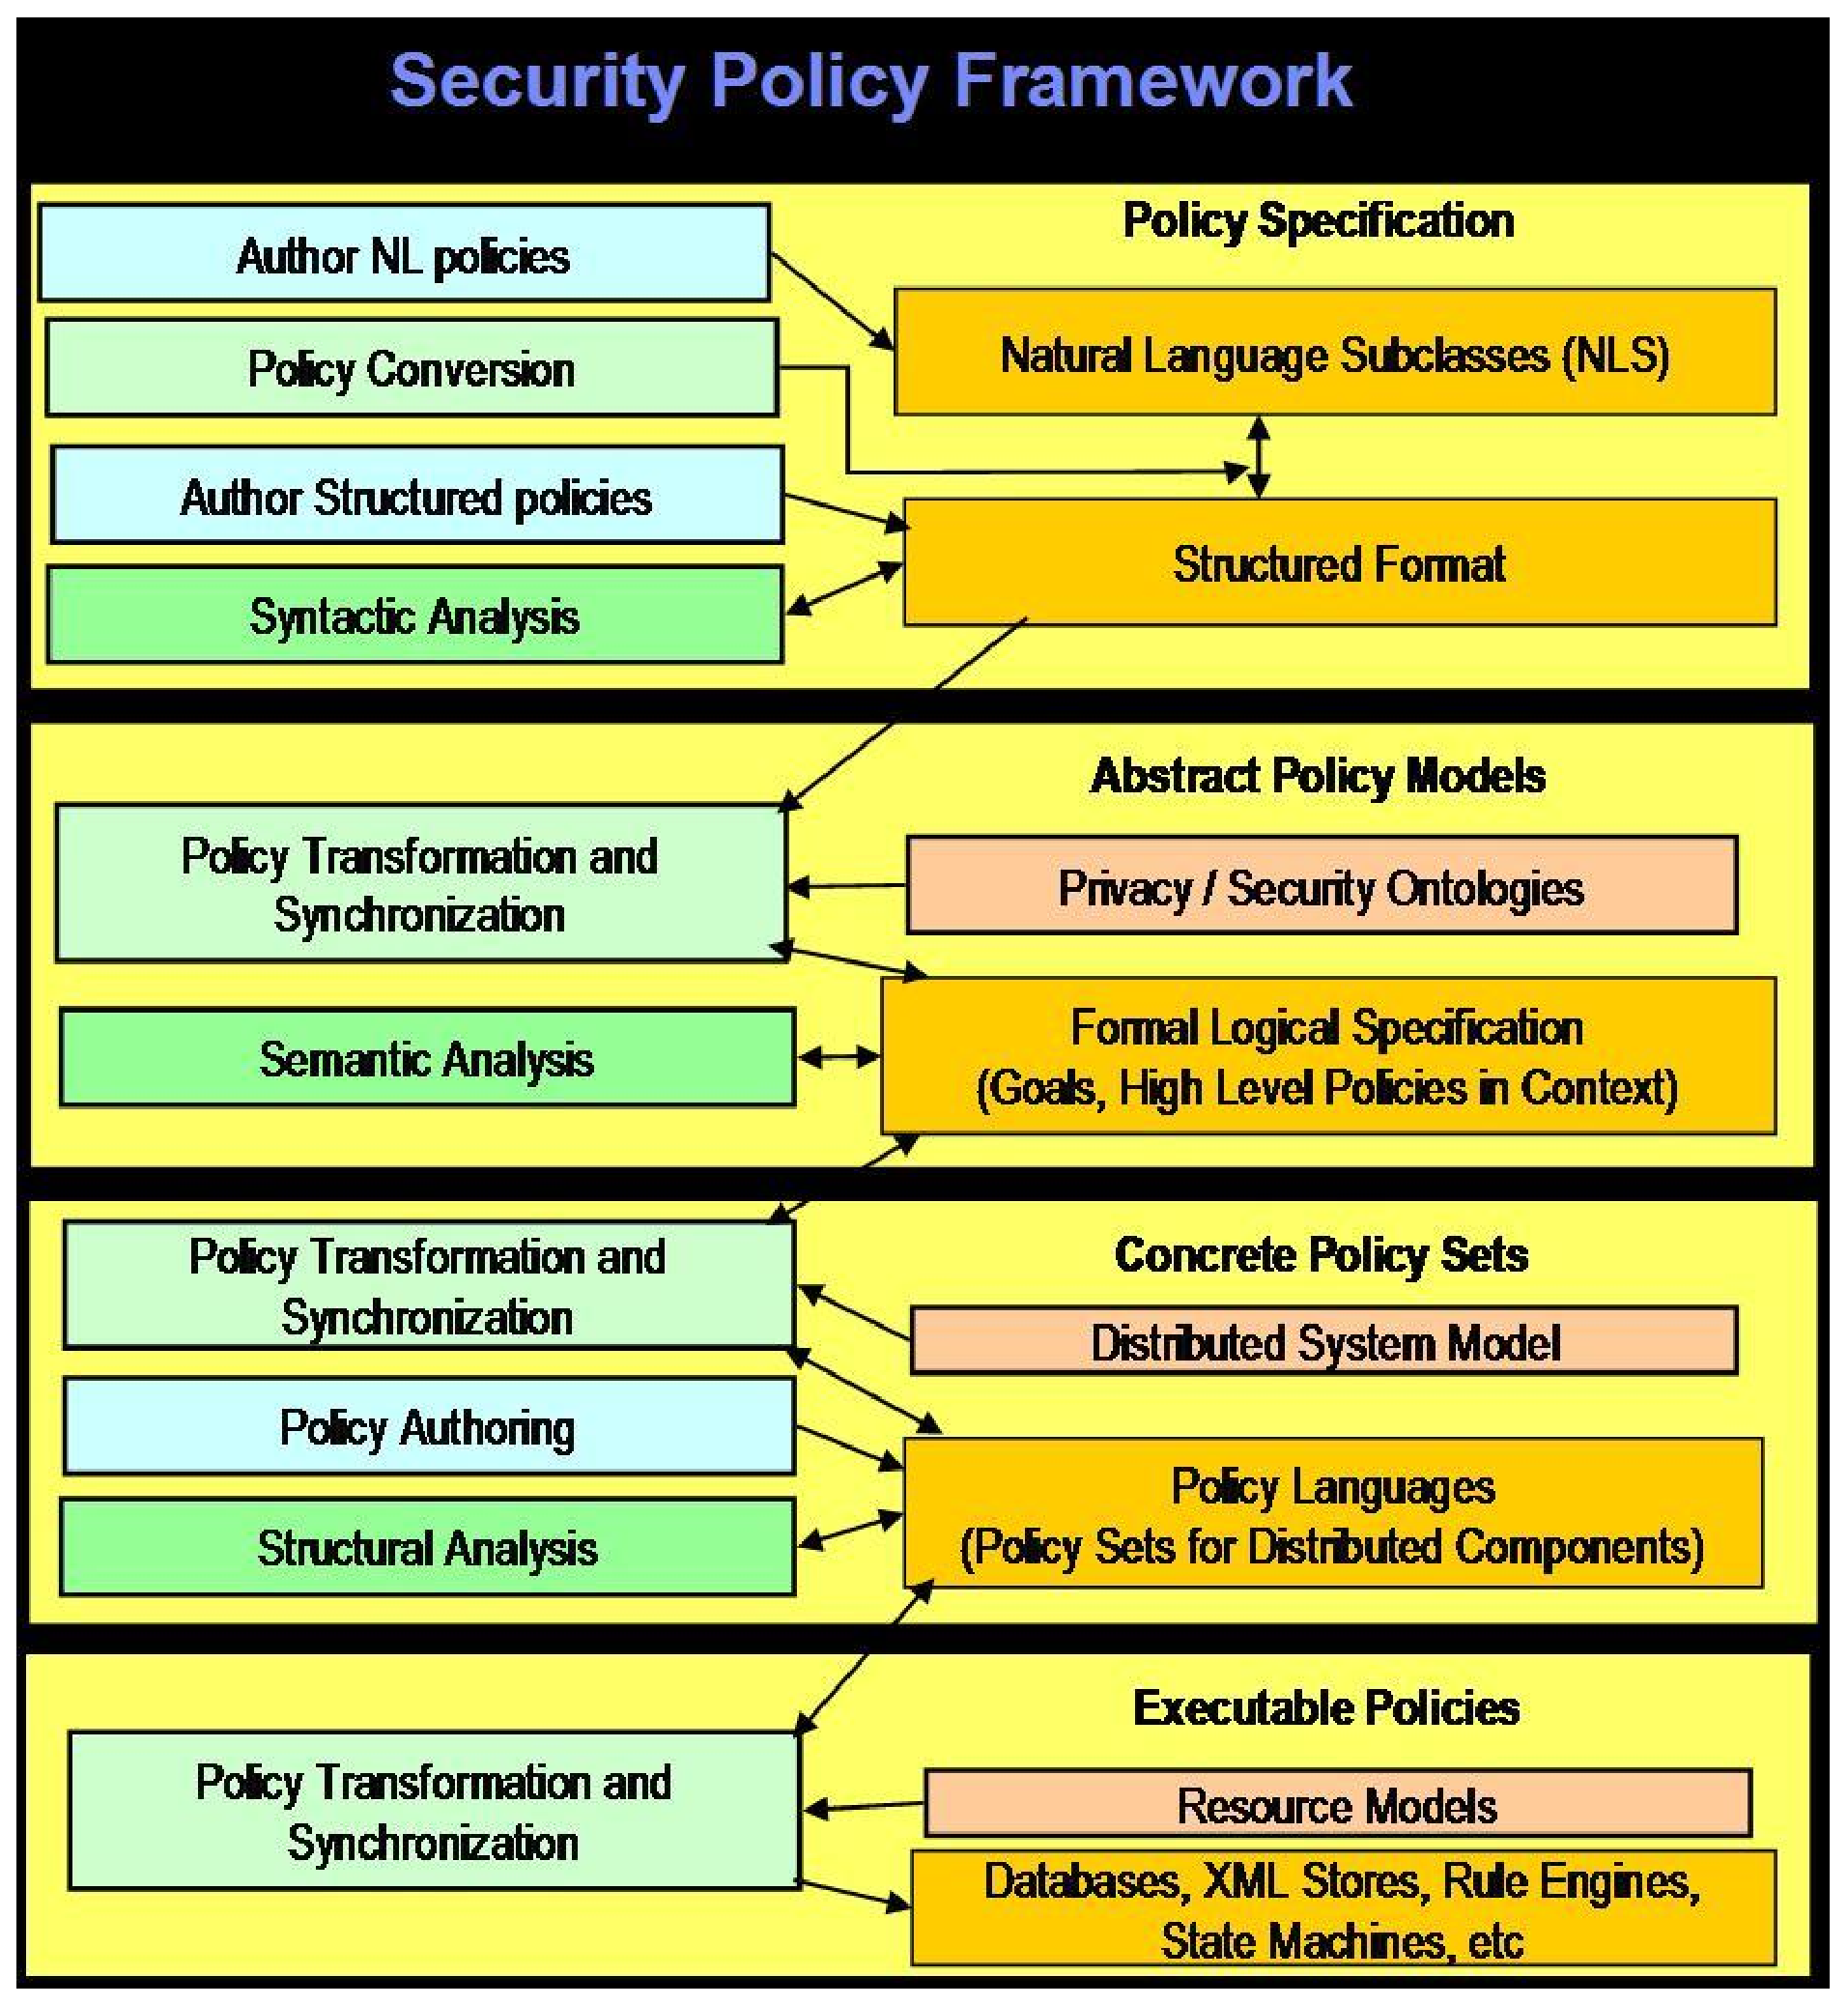
\includegraphics[width=\textwidth]{ITAPolicyModel}
 \caption{The ITA policy model~\cite{KS08}.}
 \label{fig:ITAPolicyModel}
\end{figure}
% In the following sections, we will discuss some of the issues in the
% processes in refining high-level policies into lower-level policies
% and analysing policies. 

\subsubsection{Policy refinement and policy conflict analysis}
\label{PolicyRefinementAndPolicyConflictAnalysis}
Policy refinement is the process of transforming high-level security
goals into low-level policies that can be enforced by a
system~\cite{JDM91}.  The refinement process involves the analysis of
policy conflict, policy coverage and the determination of resources
required to implement the policies~\cite{JDM91}.

One widely accepted policy refinement approach is the goal refinement
approach proposed in~\cite{RD97}. The goal refinement approach
consists of the process of identifying, recognising and instantiating
refinement patterns. Once a refinement pattern has been identified and
analysed for completeness and conflict, any policy that matches this
pattern is certain to be complete and correct. Whilst it is desirable
to have a fully automated refinement process, Moffett et al.\ argued
that it is often infeasible to do this in many situations other than
the most trivial scenarios~\cite{JDM93A}.

Policy conflict analysis is the process of verifying whether the
security policy is \emph{consistent} and
\emph{complete}~\cite{MS94}. By consistent we mean that there is no
conflict between the rules in the policies and with the capabilities
of the underlying system. By complete we mean the policy implements
all the high-level goals specified.

There are two categories of conflicts: modality conflicts and semantic
conflicts. Modality conflicts arise when the rules in the security
policies are inconsistent with one another. Modality conflicts can be
divided into the following three categories based on the types of
rules that are in conflict~\cite{EL99}:
\begin{enumerate}
\item Authorisation conflicts --- conflicts that arise because both
  positive and negative authorisation rules exist for the same action,
  subject and object tuple. In other words, a subject is
  authorised~(by the positive authorisation rule) as well as
  forbidden~(by the negative authorisation rule) to perform the same
  action on an object.
\item Obligation conflicts --- conflicts that arise because there is
  an obligation rule and a refrain~(negative obligation) rule defined
  for an action that a subject is obligated to perform as well as
  refrained from performing on an object.
\item Unauthorised obligation conflicts --- conflicts that arise
  when there are an obligation rule and a negative authorisation rule
  defined for an action that a subject is obligated but forbidden to
  perform on an object.
\end{enumerate}
Having a positive authorisation rule and a refrain rule defined for
the same action for a subject and an object is not considered as a
conflict.

Poor policy specification is not the only cause of policy
conflict. Organisation goals may be ambiguous and conflicting in
nature, e.g., maximising resource utilisation vs.\ maximising resource
availability. This will inevitably result in conflicts among policies
that are derived from it.
 
To detect these conflicts, syntactic analysis can be applied to the
policies to determine the overlap of subjects, targets and
actions~\cite{EL99}. However, the existence of overlap only reveals
the \emph{potential} modality conflict because other constraints, such
as time, might limit the applicability of the rules. Moreover,
syntactic analysis is unable to detect application-specific conflicts,
e.g., the separation of duty principle described in
Section~\ref{ClarkWilsonModel}. To detect these conflicts, the
conditions that may cause the conflicts are required to be specified
as additional constraints on the policies. The occurrence of the
conflicts may also depend on the state of the system. Analysing all
these states to check for possible conflicts is often infeasible and
therefore run-time analysis is still necessary.

Once these conflicts are detected, it is necessary to resolve
them. Jajodia et al.\ suggested a few ways to handle the conflicts
in~\cite{SJ97}. The simplest way is to do nothing but flag an error
condition. A better solution is to allow the positive authorisation
policy to override the negative authorisation policy or vice
versa. Often, the priority is given to the negative authorisation
policy based on the assumption that preventing actions would incur
less risk. Obviously this is not always true. For example, a positive
authorisation policy can be an exception to a more general negative
authorisation policy.

To alleviate this issue, priorities can be assigned to different
policies explicitly~\cite{EL99}. When conflicts arise among policies,
the highest priority policy is enforced. However, the task of priority
assignment in itself is difficult. There is also a problem of breaking
a tie if there are two or more policies with the same level of
priority. This problem is exacerbated when there are multiple parties
involved in defining and assigning policies. Inconsistency can easily
arise as each party can have different preferences. An alternative
approach is to define priority based on specificity of the
policy~\cite{AH90}. At the other extreme, meta policies are also being
proposed as a way to define the precedence relationship among
policies~\cite{EL99}. Whilst these resolution mechanisms provide more
flexibility, they also make the task of ensuring policy consistency
more complicated.  There is still no known general mechanism that is
able to detect and resolve conflicts among policies when arbitrary
conditions are allowed.

% As modern systems become more distributed, the distribution of the
% analysis procedures across the system can be problematic. The system
% can be organised in an unstructured order; each subsystem can be owned
% by different domains. This makes the policy refinement process much
% more complicated. In MANETs, subsystems can join, leave and rejoin at
% any time. This dynamic behaviour can easily cause conflicts among the
% policies.

%\subsubsection{Summary}
%\label{TopDownHierarchicalPolicyModel.Summary}
%This section presents a top-down hierarchical policy model in which
%policies are specified using high-level languages and then refined
%into low-level policies. Various issues related to the policy
%refinement process are discussed, including how conflicts among the
%policies can arise, be detected and be resolved.

\section{Summary}
\label{Review}
Recent research~\cite{JPO04} suggests that current static security
policy models are not appropriate for many modern systems, especially
when the operational environment is highly dynamic. Some models that
provide more flexibility have been
proposed~\cite{PCC07,PCC07A,JPO04}. These models are different from
the static ones in two important aspects. Firstly, the risk-benefit
tradeoff assessment on an information access request is no encoded in
the security policy itself. Instead, an explicit risk model is used in
these models to dynamically estimate the risk of an information access
request to make better informed decisions. Secondly, the new model
attempts to manage the total risk of a system as a whole, as opposed
to the risk of each access individually in the traditional
models. Users are allocated with an initial budget of risk tokens,
which they may use on their discretion to access different
information. The budget distribution is reviewed periodically based on
the benefit gained from information access of each user. However, the
models proposed are rather abstract. Many aspects of the models
require further investigation. These include the way to allocate
initial budget, the type of the market, the cost of the access, etc.

In the network management research, the top-down policy refinement
approach has received much attention recently. The idea of this
approach is to refine business goals to high-level security policies,
which in turn are refined into low-level policies
automatically. Whilst this conceptual idea is great, the current
policy conflict resolution mechanisms are still rather
primitive. There is currently no general mechanism that is able to
detect and resolve conflicts among policies when arbitrary conditions
are allowed. As modern systems become more distributed, the
distribution of the analysis procedures across the system can be
problematic. The system can be organised in an unstructured order;
each subsystem can be owned by different domains. This makes the
policy refinement process much more complicated.  In MANETs,
subsystems can join, leave and rejoin at any time. This dynamic
behaviour can easily cause conflicts among the policies.

The way we choose to approach the problem is a radical one. In this
thesis, we investigate how a specific set of decisions may be
generalised into an applicable security policy using EAs. A developed
policy inference system could be doubly useful. The generated policy
rules can be used on it own or used to verify the correctness of
existing policies. In a highly dynamic operational environment like
MANETs, where the risk factors are constantly changing, the inference
techniques must be able to dynamically update the policies inferred to
maintain their optimality. Here we explore the potential of EAs in
dynamically updating security policies with new decision
examples. Additionally, we observe that the risk-budget based policy
models reviewed in Section~\ref{FlexibleAccessControlModels} are
really families of policies. Each instance in a policy family
constrains the system and therefore affects the operational behaviour
and effectiveness of the system in its own way. We introduce the
notion of mission-specific policy and demonstrate how EAs can be used
to search for the~(near) optimal policies that fit a specific set of
missions using simulation runs~(instead of a set of decision
examples).

\section{Conclusions}
\label{SecurityPolicy.Conclusion}
This chapter summarises various influential security policies and
models in the literature. It then introduces the top-down hierarchical
policy model in which allows policies to be specified using high-level
languages and then refined into low-level policies. Various issues
related to the policy refinement and conflict analysis process are
discussed. Lastly, it reviews the current state of the art in security
policy development and reiterates the research objectives of the
thesis.


% ------------------------------------------------------------------------


%%% Local Variables: 
%%% mode: latex
%%% TeX-master: "../thesis"
%%% End: 
